\documentclass[11pt, letterpaper]{article}
\pagestyle{empty}
\usepackage[a4paper, margin=1cm]{geometry} % Adjust margins as needed
\usepackage{multirow}
\usepackage{enumitem}
\usepackage{graphicx}
\usepackage{minted}
\usepackage[most]{tcolorbox}
\usepackage{etoolbox}
\usepackage[table]{xcolor}
\usepackage{tabularx}
\usepackage{microtype}
\usepackage{tikz}
\usepackage[md]{titlesec}
\setminted{fontsize=\large}
\usemintedstyle{bw}
\newcommand{\includeminted}[3]
{
  \begin{center}
  \textbf{#1}
  \vspace{-5pt}
  \inputminted[linenos, breaklines]{#2}{#3}
  \end{center}
}

\newcommand{\mintbox}[3]
{
  \begin{center}
  \textbf{#1}
  \vspace{-5pt}
  \begin{tcolorbox}
  \inputminted[]{#2}{#3}
  \end{tcolorbox}
  \end{center}
}

\title{Exam revision}
\author{}
\date{}

\begin{document}
\normalsize
\section{Lab 10}
\includeminted{Figure 1: Array.h}{cpp}{../10/src/Array.h}
\clearpage
\section{Lab 11}
\includeminted{Figure 2: DoublyLinkedList.h}{cpp}{../11/src/DoublyLinkedList.h}
\clearpage
\includeminted{Figure 3: DoublyLinkedListIterator.h}{cpp}{../11/src/DoublyLinkedListIterator.h}
\clearpage
\section{Lab 12}
\includeminted{Figure 4: BTree.h}{cpp}{../12/src/BTree.h}
\clearpage
\includeminted{Figure 5: TreeDecorator.h}{cpp}{../12/src/TreeDecorator.h}
\clearpage
\section{Lab 8 - optional}
\includeminted{Figure 6: DynamicStack.h}{cpp}{../8/src/DynamicStack.h}
\clearpage
\section{Lab 6 - optional}
\includeminted{Figure 7: ArraySorter.h}{cpp}{../6/src/ArraySorter.h}
\clearpage
\includeminted{Figure 8: BubbleSorter.h}{cpp}{../6/src/BubbleSorter.h}
\clearpage
\section*{Revision Questions}
\setlength{\parskip}{0.5em}

\newtcolorbox{answerspace}{
  colback=white,
  colframe=black,
  boxrule=0.5pt,
  left=2mm,
  right=2mm,
  top=1mm,
  bottom=1mm,
  enhanced,
  height=3cm,
  breakable
}

\begin{enumerate}[leftmargin=*, label=\textbf{\arabic*.}]
  \item What is the difference between a shallow copy and a deep copy?
    \begin{answerspace}
    \end{answerspace}

  \item Why should you use \texttt{make\_shared} and \texttt{make\_unique} when using smart pointers?
    \begin{answerspace}
    \end{answerspace}

  \item What is the point of \texttt{perfect forwarding}, and why should you use \texttt{std::forward} to forward arguments?
    \begin{answerspace}
    \end{answerspace}

  \item Give all the function signatures of a \texttt{Node} class, and where it could be used for a copy constructor, copy assignment operator, move constructor and move assignment operator.
    \begin{answerspace}
    \end{answerspace}

  \item Explain mutually dependent classes in C++ and give an example.
    \begin{answerspace}
    \end{answerspace}

  \item What are the dangers of using circular references with \texttt{shared\_ptr}?
    \begin{answerspace}
    \end{answerspace}
\clearpage
  \item How can we construct a tree where all nodes have the same degree?
    \begin{answerspace}
    \end{answerspace}

  \item What is the difference between l-value references and r-value references?
    \begin{answerspace}
    \end{answerspace}

  \item What is a key concept of abstract data types?
    \begin{answerspace}
    \end{answerspace}

  \item What must a value-based data type define in C++?
    \begin{answerspace}
    \end{answerspace}

  \item What is an object adapter?
    \begin{answerspace}
    \end{answerspace}

  \item What is the difference between copy constructor and assignment operator and how do we guarantee safe function?
    \begin{answerspace}
    \end{answerspace}
    
    \clearpage

  \item What is the best-case, worst-case and average case lookup in a binary tree?
    \begin{answerspace}
    \end{answerspace}

  \item What are reference data members and how do we initialize them?
    \begin{answerspace}
    \end{answerspace}

  \item What is RAII and how is it leveraged in C++?
    \begin{answerspace}
    \end{answerspace}

  \item What is the slowest time order?
    \begin{answerspace}
    \end{answerspace}

  \item What is Amortized Analysis?
    \begin{answerspace}
    \end{answerspace}

  \item What is the time complexity of a stack push?
    \begin{answerspace}
    \end{answerspace}

  \item What is the time complexity of a stack pop?
    \begin{answerspace}
    \end{answerspace}

  \item What is the time complexity of pop(k), where k = num elements to pop?
    \begin{answerspace}
    \end{answerspace}

  \item How do you use aggregate method for calculating amortized cost?
    \begin{answerspace}
    \end{answerspace}

  \item How do you use aggregate method for calculating amortized cost?
    \begin{answerspace}
    \end{answerspace}

  \item What is the Amortized cost of pop(k)?
    \begin{answerspace}
    \end{answerspace}

  \item How do you calculate load factor?
    \begin{answerspace}
    \end{answerspace}

  \item How can you implement queue with an Array?
    \begin{answerspace}
    \end{answerspace}

  \item What is a sentinel object/node?
    \begin{answerspace}
    \end{answerspace}

  \item What data structure would you use to perform DFS?
    \begin{answerspace}
    \end{answerspace}

  \item What data structure would you use to perform BFS?
    \begin{answerspace}
    \end{answerspace}

  \item What is a frontier node?
    \begin{answerspace}
    \end{answerspace}

  \item How to implement post-order with stack?
    \begin{answerspace}
    \end{answerspace}

  \item How to implement in-order with stack?
    \begin{answerspace}
    \end{answerspace}

  \item How to insert a number into a BST?
    \begin{answerspace}
    \end{answerspace}

  \item How to delete a number in BST?
    \begin{answerspace}
    \end{answerspace}

  \item What type of tree traversal yields sorted values in BST?
    \begin{answerspace}
    \end{answerspace}

\end{enumerate}
\clearpage
\section*{Tree Traversal Practice}

\noindent\textbf{Instructions:}  
For each tree below, write the \textbf{node number} inside each circle according to the specified traversal order.

\vspace{1em}

\begin{enumerate}[leftmargin=*]
  \item \textbf{Pre-order traversal:} Number the nodes in pre-order.
  \item \textbf{In-order traversal:} Number the nodes in in-order.
  \item \textbf{Post-order traversal:} Number the nodes in post-order.
\end{enumerate}

\vspace{2em}

% Tree A
\newcommand{\binarytree}{
\begin{center}
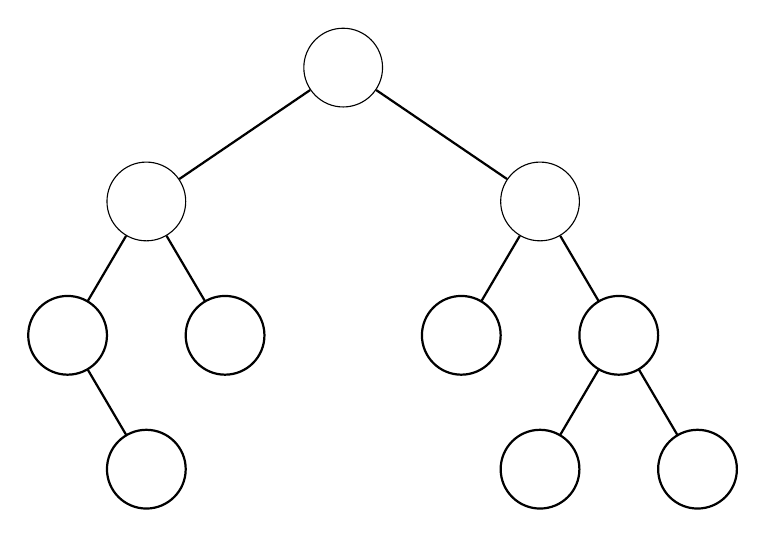
\begin{tikzpicture}[level distance=1.7cm,
  level 1/.style={sibling distance=5cm},
  level 2/.style={sibling distance=2cm},
  every node/.append style={circle,draw,minimum size=1cm, font=\large, fill=white, text=black},
  edge from parent/.style={draw,thick}]
\node {} % root
  child { node {} 
    child { node {} 
      child[missing]
      child { node {} } 
    }
    child { node {} } 
  }
  child { node {} 
    child { node {} } 
    child { node {} 
      child { node {} } 
      child { node {} } 
    }
  };
\end{tikzpicture}
\end{center}
}

% Tree B
\newcommand{\binarytreeA}{
\begin{center}
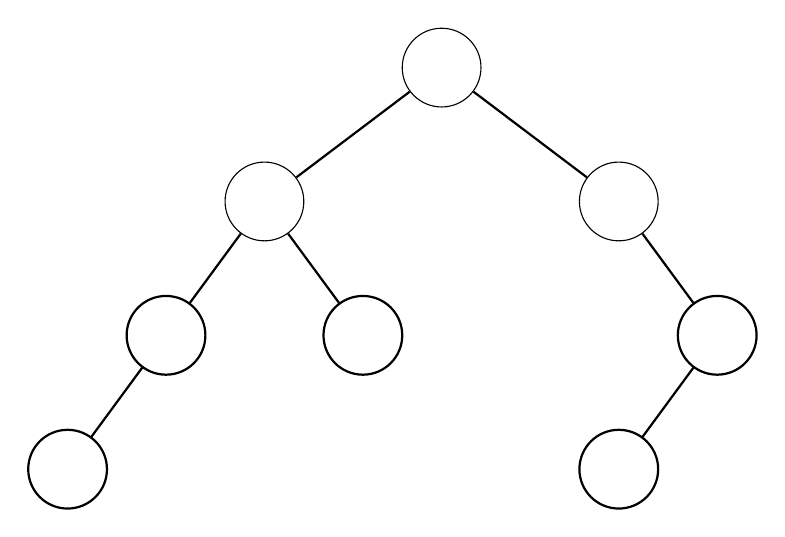
\begin{tikzpicture}[level distance=1.7cm,
  level 1/.style={sibling distance=4.5cm},
  level 2/.style={sibling distance=2.5cm},
  every node/.append style={circle,draw,minimum size=1cm, font=\large, fill=white, text=black},
  edge from parent/.style={draw,thick}]
\node {}
  child { node {}
    child { node {} 
      child { node {} } 
      child[missing] 
    }
    child { node {} }
  }
  child { node {}
    child[missing]
    child { node {} 
      child { node {} }
      child[missing]
    }
  };
\end{tikzpicture}
\end{center}
}

% Tree C
\newcommand{\binarytreeB}{
\begin{center}
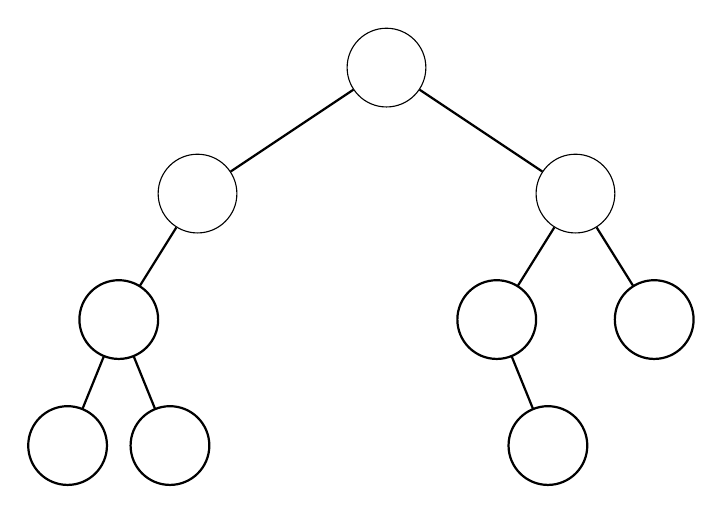
\begin{tikzpicture}[level distance=1.6cm,
  level 1/.style={sibling distance=4.8cm},
  level 2/.style={sibling distance=2cm},
  level 3/.style={sibling distance=1.3cm},
  every node/.append style={circle,draw,minimum size=1cm, font=\large, fill=white, text=black},
  edge from parent/.style={draw,thick}]
\node {}
  child { node {}
    child { node {} 
      child { node {} } 
      child { node {} } 
    }
    child[missing]
  }
  child { node {} 
    child { node {} 
      child[missing] 
      child { node {} }
    }
    child { node {} }
  };
\end{tikzpicture}
\end{center}
}

% Pre-order Tree
\subsection*{1. Pre-order Traversal}
\binarytree
\binarytreeA
\binarytreeB
\vspace{1.5cm}


% In-order Tree
\subsection*{2. In-order Traversal}
\binarytree
\binarytreeA
\binarytreeB
\vspace{1.5cm}

\clearpage

% Post-order Tree
\subsection*{3. Post-order Traversal}
\binarytree
\binarytreeA
\binarytreeB

% Massive tree diagram + structural analysis questions
\clearpage
\section*{Tree Analysis Practice}

\noindent
\textbf{Instructions:} Use the tree diagram below to answer the following questions about its structure.

\vspace{1em}

% Massive Tree
\begin{center}
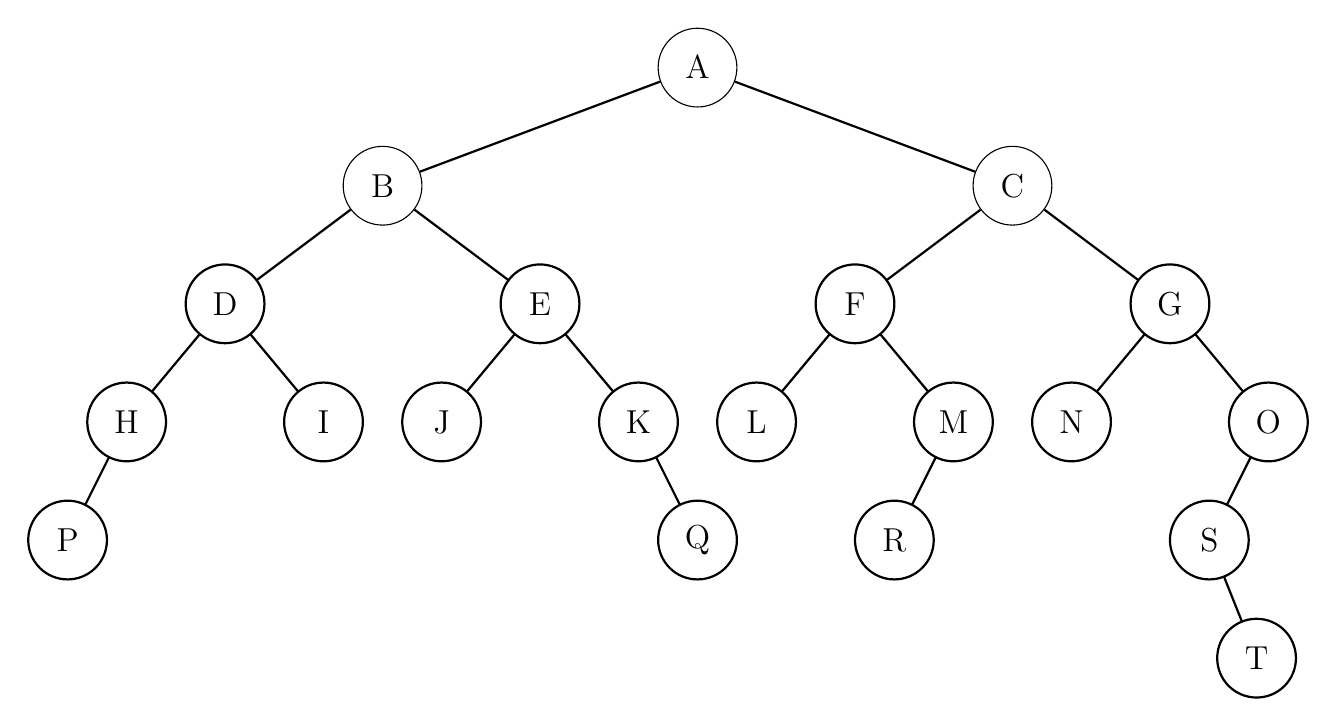
\begin{tikzpicture}[level distance=1.5cm,
  level 1/.style={sibling distance=8cm},
  level 2/.style={sibling distance=4cm},
  level 3/.style={sibling distance=2.5cm},
  level 4/.style={sibling distance=1.5cm},
  level 5/.style={sibling distance=1.2cm},
  level 6/.style={sibling distance=1cm},
  every node/.append style={circle,draw,minimum size=1cm, font=\large, fill=white, text=black},
  edge from parent/.style={draw,thick}]
\node {A} % root
  child { node {B}
    child { node {D}
      child { node {H}
        child { node {P} }
        child[missing]
      }
      child { node {I} }
    }
    child { node {E}
      child { node {J} }
      child { node {K}
        child[missing]
        child { node {Q} }
      }
    }
  }
  child { node {C}
    child { node {F}
      child { node {L} }
      child { node {M}
        child { node {R} }
        child[missing]
      }
    }
    child { node {G}
      child { node {N} }
      child { node {O}
        child { node {S}
          child[missing]
          child { node {T} }
        }
        child[missing]
      }
    }
  };
\end{tikzpicture}
\end{center}

\vspace{1em}

\begin{enumerate}[leftmargin=*, label=\textbf{\arabic*.}]
  \item What is the \textbf{root node}?
  \item List all the \textbf{leaf nodes}.
  \item What is the \textbf{degree} of node B?
  \item What is the \textbf{degree} of node G?
  \item What is the \textbf{depth} of node L?
  \item What is the \textbf{height} of node B?
  \item What is the \textbf{height} of the entire tree?
  \item How many \textbf{edges} are in the tree?
  \item What is the \textbf{path length} from A to M?
  \item What is the \textbf{total number of nodes} in the tree?
  \item How many \textbf{internal nodes} (nodes that are not leaves) are there?
  \item Which node has the \textbf{maximum degree}?
  \item What is the \textbf{subtree rooted at E}?
  \item What is the \textbf{minimum number of levels} needed to fit this tree?
  \item What type of \textbf{tree traversal} would visit the nodes in the order: A, B, D, H, P, I, E, J, K, Q, C, F, L, M, R, G, N, O, S, T?
\end{enumerate}
\end{document}
